% Copyright (c) 2014,2016 Casper Ti. Vector
% Public domain.
\chapter{KV Framework设计}
% \pkuthssffaq % 中文测试文字。
% vim:ts=4:sw=4
\section{概览}\label{sec:req}
	这部分将介绍键值对框架(Key Value Framework)的概念、概述以及接口的定义。KVF定义了统一的数据模型、函数和参数。通过这样一个框架,不同的Key value storage可以注册和注销注册,像虚拟文件系统管理ext3、jfs一样。此外该框架提供了统一的API以便上层应用调用,从而避免了同一个应用为了在不同厂商的的KV store实现功能而开发多个适配器的情况。

\section{键值存储(Key Value Store)介绍}\label{sec:doc-dir}
	

		传统的存储系统是基于SCSI架构的,客户端使用逻辑块地址(Logical Block Address,LBA)进行读写数据。在块的基础上我们可以提供更多的服务,比如文件系统、数据库等等。作为替代品,键值存储(也称为目标存储系统)提供了键值对操作。上层应用通过指定键名来存储数据值,键的名字可以是一个字符串变量,数据值可以是一个数据缓冲变量,这样上层应用可以很容易地存储数据,不需要基于线性块空间的复杂的布局设计,只需要聚焦于键名策略的设计和如何存储键名(比如使用分布式哈希表存储)。基于键值存储我们可以很容易地构造文件、swift、hdfs、no-sql甚至是块服务,如图1所示。
	\begin{center}
		\includegraphics[width=13.9cm]{img/figure1.pdf}
	\end{center}
	\centerline {图1}
	%\includepdf{figure1.pdf}
	%\epsfig{figure=figure1,height=6.4cm}
	
		实际上512或者4096字节大小的块设备是一种简单的键值存储,它的键名是LBA(Logical Block Address),数据值是512或者4096个字节大小的数据,因为这种简单性,上层应用需要复杂的布局设计(比如RamCloud),而数据大小可变的键值存储更加灵活,所以上层应用可以很容易在上面存储数据,这是一种性能和可用性之间的权衡。根据冗余的多少,键值存储可以分为三类:
	\begin{itemize}
		\item \textbf{独立的KVS}:
		
			独立的KVS是指如下的应用场景:
			应用客户端直接从一个独立的设备读写数据,比如从一个单独的硬盘、闪存卡等等。相关的产品包括希捷的Kineitic以及闪迪的Fusionio等等

		\item \textbf{分布式KVS}:
		
			分布式KVS是指如下应用场景:
			数据储存在多个服务器节点之间存在冗余,通过某种方式相互通信从而将这些服务器节点的存储资源整合到一起,并应用客户端提供读写接口。相关产品包括Ceph、mongoDB等等。

		\item \textbf{多数据中心的KVS}:
		
			多数据中心的KVS应用于如下场景:
			数据在多重数据中心都有冗余,有复制备份和纠删码的特性,相关的产品包括Amazon S3、SWIFT等等。
	\end{itemize}

		这三种KVS是有关联的,但是可以相互独立,例如多数据中心的KVS可以是基于分布式KVS的,分布式KVS页可以是基于独立KVS的。
\section{Key Value Framework (KVF) 数据模型}\label{sec:KVF-model}
	通过Key Value Framework(KVF)不同的厂商可以通过注册自己的Key Value库(KV-LIB)来管理它的Key Value Storage(KVS)。 这些KV-LIB应该遵循KVF数据模型,KVS提供pool,pool提供对象。pool支持嵌套设计,这意味着一个pool可以在另一个pool的上面,如图2所示。
	\begin{center}
		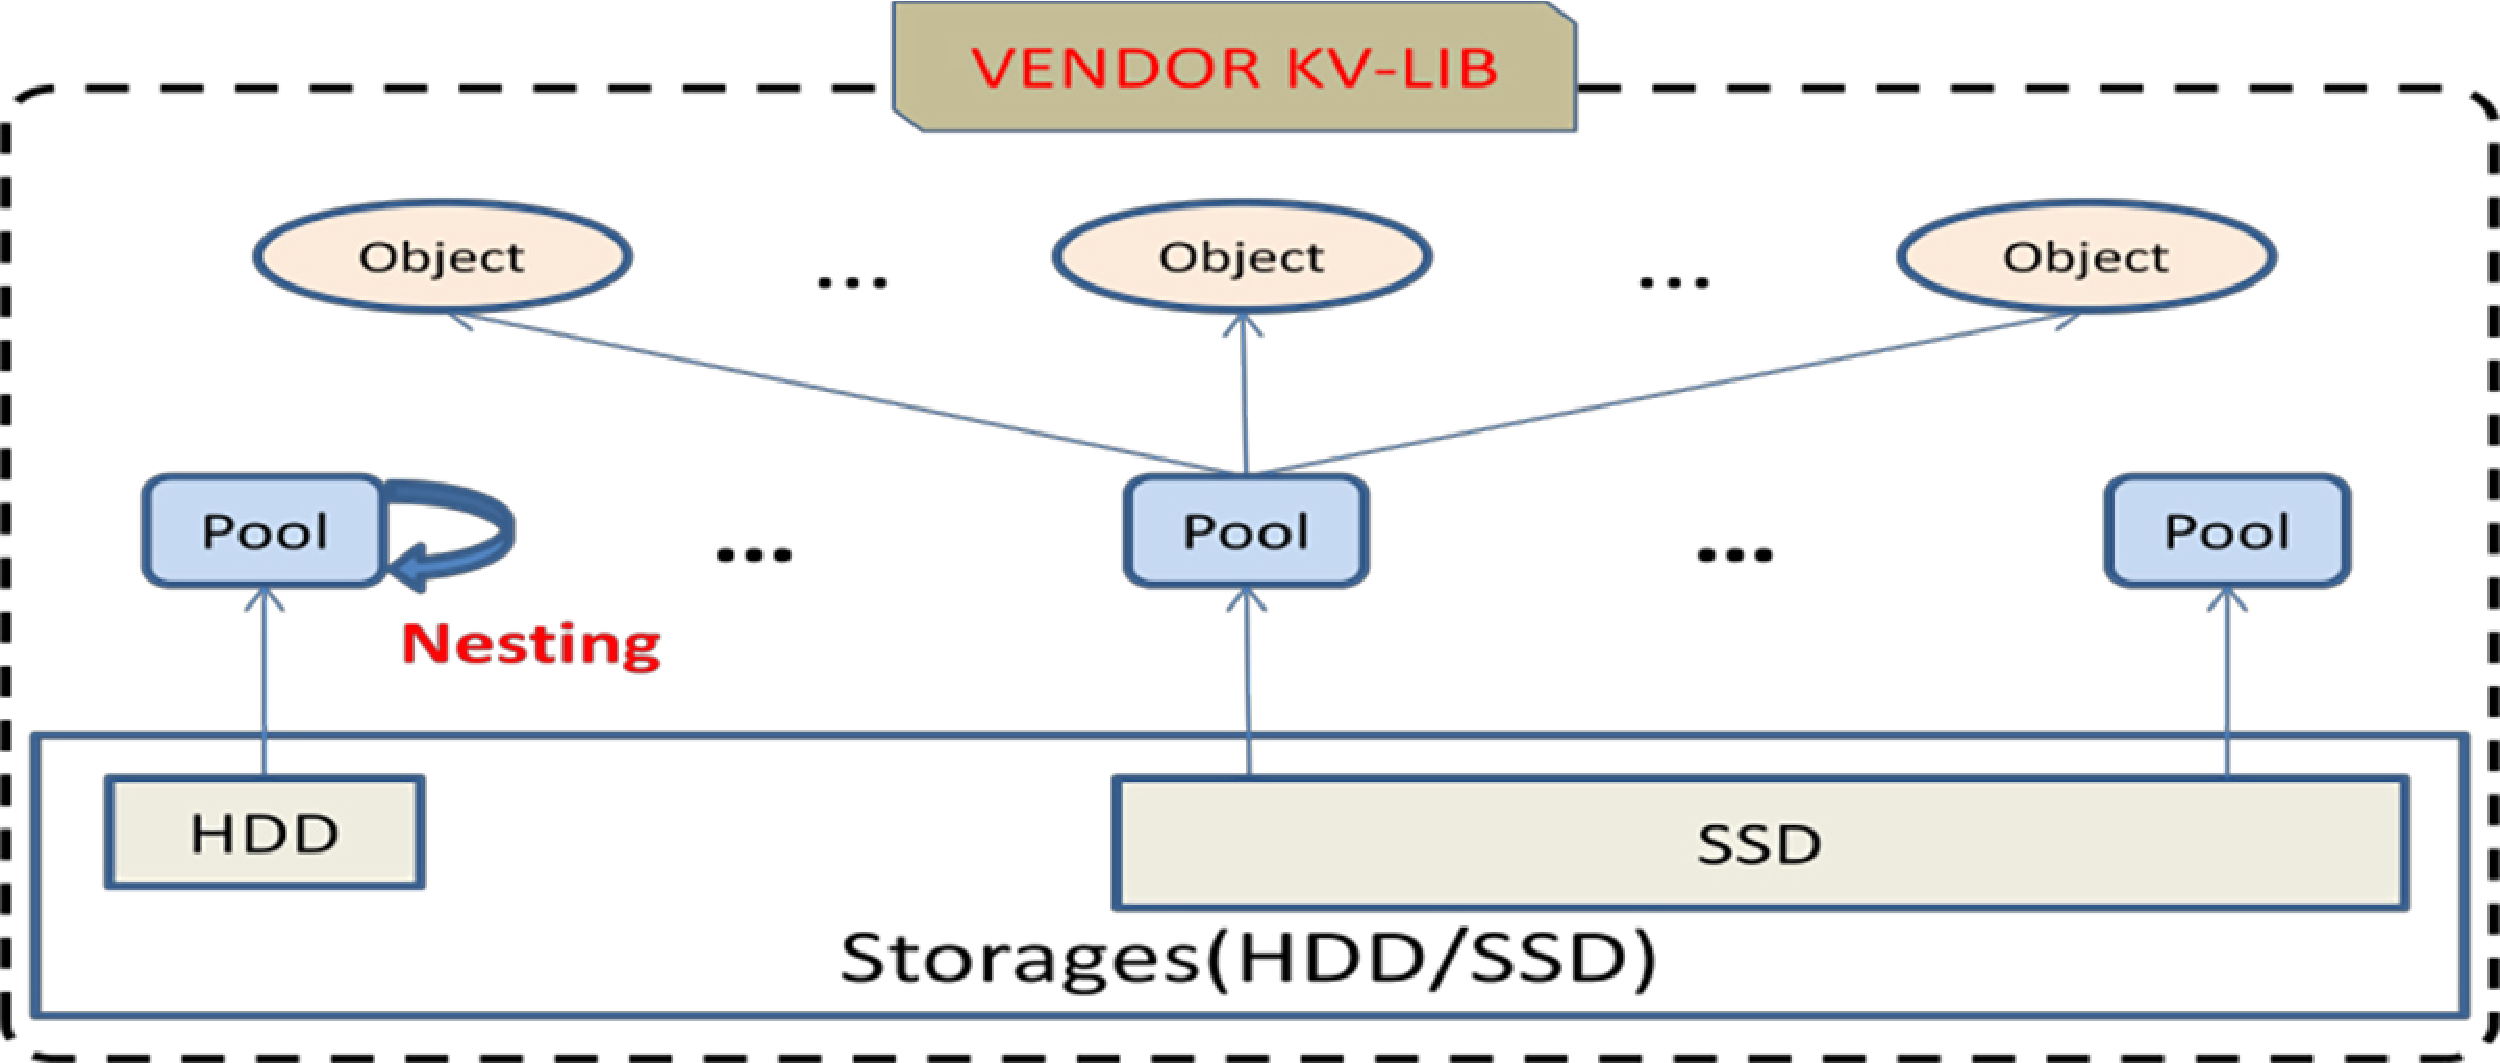
\includegraphics[width=13.9cm]{img/figure2.pdf}
	\end{center}
	\centerline {图2}

\section{Key Value Framework (KVF) 体系结构}\label{sec:KVF-Architecture}
	KVF提供了两层接口:底层管理接口(Lower Layer Manage API)和上层访问接口(Upper Layer Access API)。如图3所示
	\begin{center}
		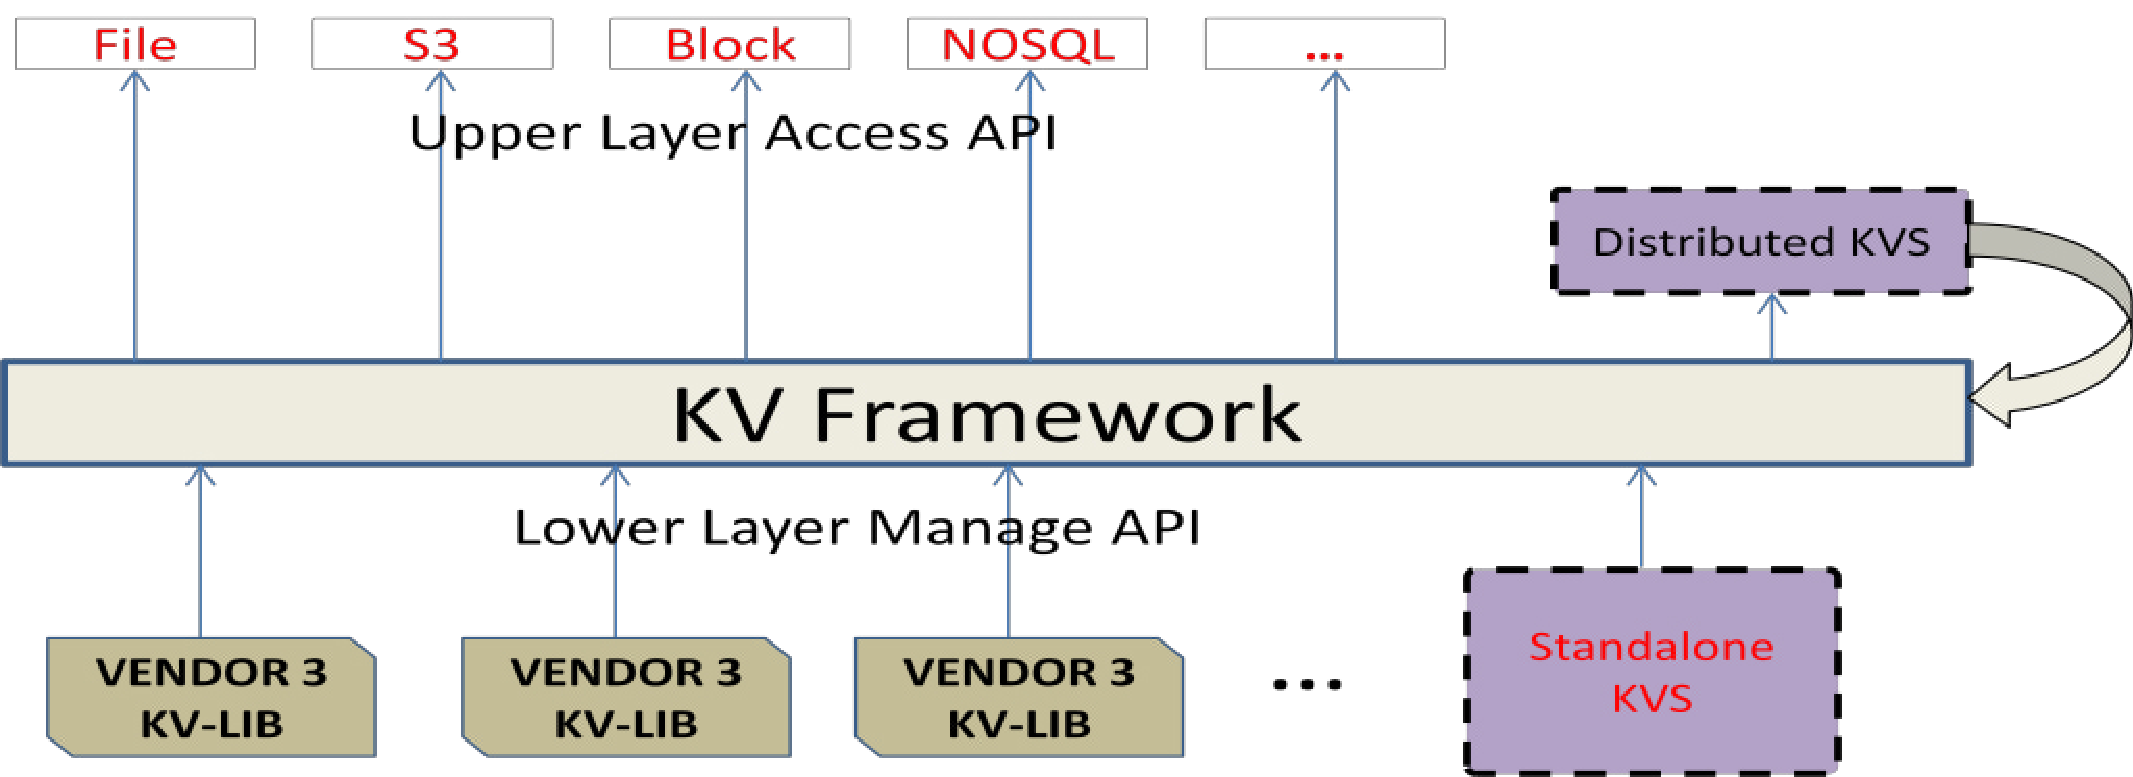
\includegraphics[width=13.9cm]{img/figure3.pdf}
	\end{center}
	\centerline {图3}
	底层管理提供注册和注销函数,共有三种接口:对象接口,Pool接口和KV-LIB接口。
	上层访问提供统一的键值接口,从而使上层应用程序变得简单并有更强的兼容性。
	此外一些应用可以通过利用基于其他KVS的上层访问接口提供键值服务,然后再重新注册到KVF中,这样就使得嵌套设计变得容易。
% \section{Key Value Framework (KVF) 底层管理接口}\label{sec:KVF-Lower-Layer-Manage-API}
% 	这节将描述底层管理接口设计,包括KVF接口,Pool接口,对象接口。KVF的相关函数名称都以“KVF\_”开始。
% 	\subsection{基本数据结构}
% 		基本数据类型定义
% 		\begin{center}
% 			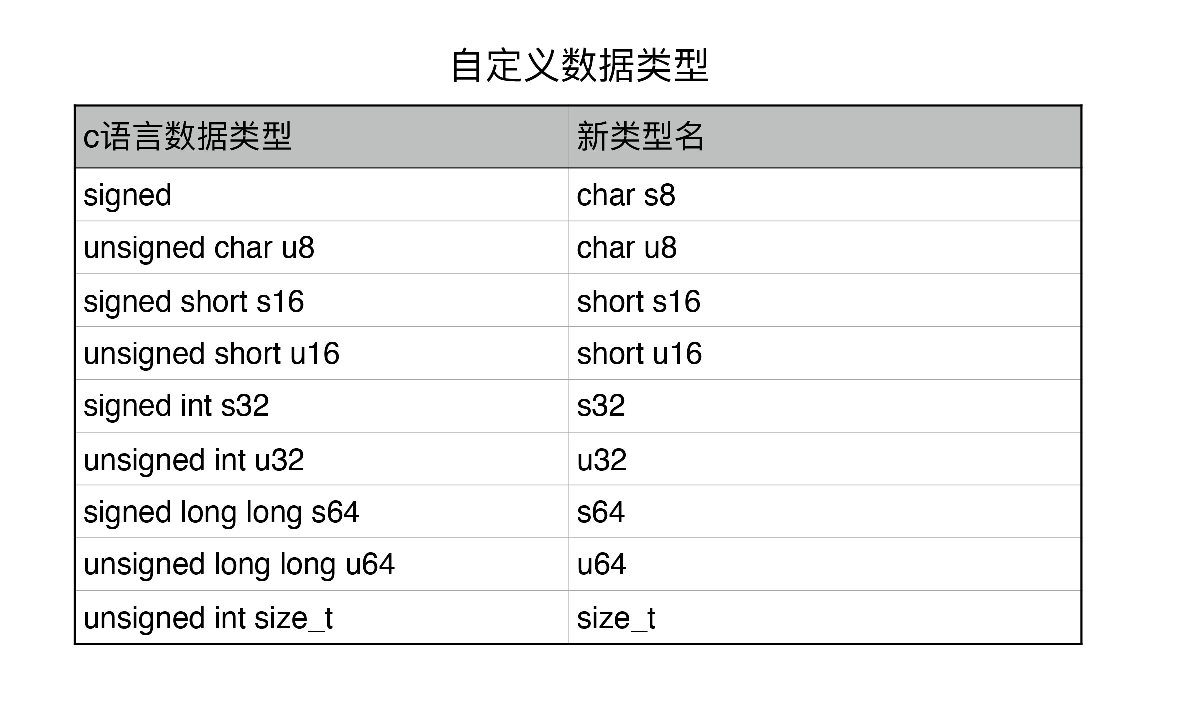
\includegraphics[width=13.9cm]{img/figure4.pdf}
% 		\end{center}

% 		字符串结构定义
% 		\begin{center}
% 			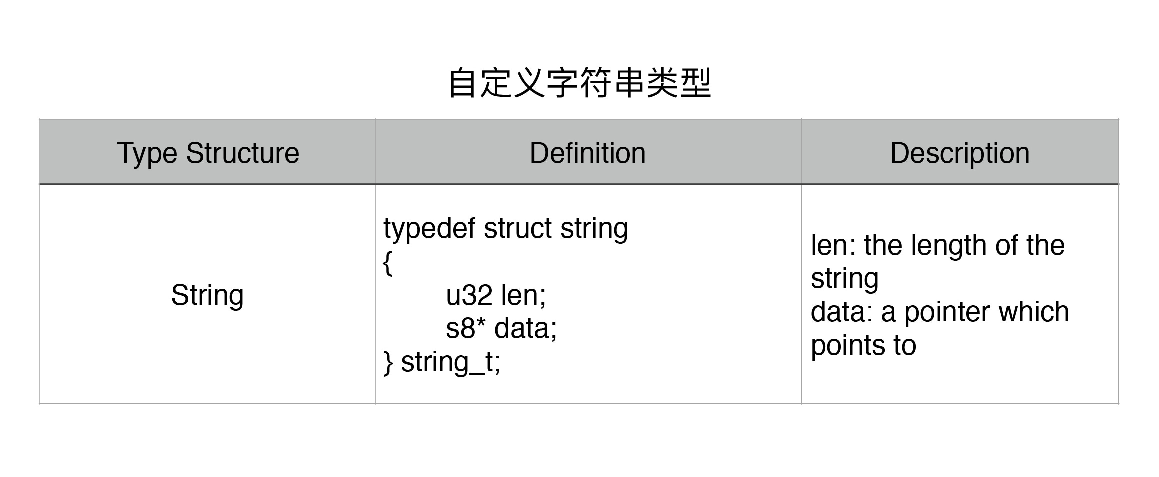
\includegraphics[width=13.9cm]{img/figure5.pdf}
% 		\end{center}



